% Auriga theme
% https://github.com/anishathalye/auriga

\documentclass[14pt,aspectratio=169]{beamer}
\usepackage{pgfpages}
\usepackage{fancyvrb}
\usepackage{booktabs,dcolumn}
\usepackage{tikz}
\usetikzlibrary{arrows.meta, positioning, quotes}
\usepackage{pgfplots}

% \ifnotes
% \setbeamertemplate{note page}[plain]
% \setbeameroption{show notes on second screen=right}
% \fi

\usetheme{auriga}
\usecolortheme{auriga}

% define some colors for a consistent theme across slides
\definecolor{red}{RGB}{181, 23, 0}
\definecolor{blue}{RGB}{0, 118, 186}
\definecolor{gray}{RGB}{146, 146, 146}

\title{Historia Económica Argentina}

\author{\underline{Sebastián Freille} \inst{1}}

\institute[shortinst]{\inst{1} IEF-UNC \\ UCC}
\date{}

\AtBeginSection[]{
    \begin{frame}
    \vfill
    \centering
    \begin{beamercolorbox}[sep=8pt,center,shadow=true,rounded=true]{title}
        \usebeamerfont{title}\insertsectionhead\par%
    \end{beamercolorbox}
    \vfill
    \end{frame}
}



\AtBeginSubsection[]{
    \begin{frame}
    \vfill
    \centering
    \begin{beamercolorbox}[sep=6pt,center,shadow=true,rounded=true]{title}
        \usebeamerfont{title}\insertsubsectionhead\par%
    \end{beamercolorbox}
    \vfill
    \end{frame}
}


\AtBeginSubsubsection[]{
    \begin{frame}
    \vfill
    \centering
    \begin{beamercolorbox}[sep=4pt,center,shadow=true,rounded=true]{title}
        \usebeamerfont{title}\insertsubsubsectionhead\par%
    \end{beamercolorbox}
    \vfill
    \end{frame}
}


\begin{document}

{
  % rather than use the frame options [noframenumbering,plain], we make the
  % color match, so that the indicated page numbers match PDF page numbers
  \setbeamercolor{page number in head/foot}{fg=background canvas.bg}
  \begin{frame}
    \titlepage
  \end{frame}
}

  
  \section{Capítulo 1. El período de progreso}

  \subsection{El sistema de Caja de Conversión}


   \begin{frame}\frametitle{Un período de reformas institucionales y políticas}
    \begin{itemize}\itemsep 10pt
      \item Es importante resaltar que aún a pesar de la crisis, los
        primeros signos de un cambio en la política fueron dados con
        la asunción de Pellegrini
        \item Si bien el diagnóstico era compartido --necesidad de desinflación y
          estabilización- no sucedía lo mismo con las políticas a
          seguir. Reflejaba condicionamientos
          politicos y sociales
        \item En el frente fiscalm fueron
            importantes las nuevas medidas de 1891: 1)
            aranceles a las M pagaderas en pesos oro; 2) impuesto
            ad-valorem sobre X de principales commodities
       \end{itemize}
      \end{frame}


 \begin{frame}\frametitle{Reformas fiscales}
    \begin{itemize}\itemsep 10pt
      \item El principal problema de estas reformas fiscales fue el
        \textit{timing} $\longrightarrow$ ``too little, too late''
        \item Dada la acelerada depreciación real del peso papel, los
          recursos fiscales bajaron fuertemente al caer abruptamente
          las M --lograr un presupuesto equilibrado en 1891 resultaba
          imposible sin un enorme sacrificio de gasto
          \item Al mismo tiempo, el defícit subía al subir el gasto en
            pesos papel de servicios de la deuda --pagos de 11.4 mill
            (1890) y 11.6 mill (1891) representaban 25\% del gasto
            total (1890) y 34\% del gasto total (1891)!
            $\longrightarrow$ efecto depreciación
       \end{itemize}
      \end{frame}
      


       \begin{frame}\frametitle{Reformas fiscales (cont.)}
\begin{figure}[htbp]\vspace{0cm}
  \centering
  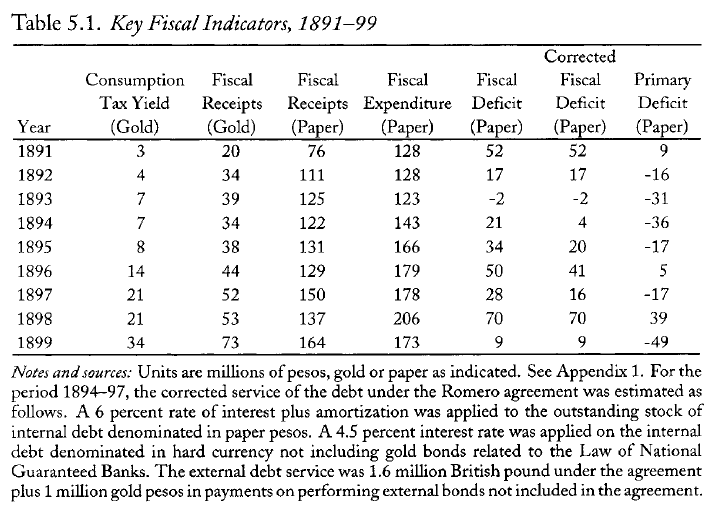
\includegraphics[scale=0.55]{uni1_fis05}
  \caption[bpe]{Principales indicadores fiscales, 1891-99. Fuente:
    Della Paolera and Taylor (2001)}
  \label{fig:uni1_01}
\end{figure} 
  \end{frame}



  


      
  
  \begin{frame}\frametitle{El nuevo modelo monetario}
    \begin{itemize}\itemsep 10pt
      \item Luego de la debacle del sistema bancario y de la crisis
        económica de 1890-91 el gobierno de Pellegrini se vió obligado
        a refundar el modelo monetario
\item Sistema inspirado en el modelo inglés $\longrightarrow$
  originalmente sistema mixto --metalico y fiduciario- con un banco a
  cargo de la
  emisión en Londres y regiones aledañas (Banco de Inglaterra, BdI) y
  bancos del interior emitiendo billetes propios usando como reservas
  billetes del Banco de Inglaterra
  \item Frecuentes corridas cambiarias en Inglaterra estimularon el
    debate entre la \textit{Currency School} y la \textit{Banking School}
       \end{itemize}
      \end{frame}


      \begin{frame}\frametitle{El nuevo modelo monetario (cont.)}
    \begin{itemize}\itemsep 10pt
      \item El Acta de Peel (1844) zanjó la cuestión en favor de la
        \textit{Currency School} $\longrightarrow$ se dividió al BdI
        de Inglattera en departamento de \textbf{emision} y
        \textbf{comercial}.
        \item Monopolio de emisión del BdI pero $\longrightarrow$ sólo
          podía emitir contra entrada de oro y debía retirar billetes
          cuando salía oro.
          \item Argentina emuló estas reformas y creó dos organismos:
            1) la Caja de Conversión (1890) y 2) el Banco de la Nación
            Argentina (BNA, 1891)
       \end{itemize}
      \end{frame}


 \begin{frame}\frametitle{La Caja de Conversión}
    \begin{itemize}\itemsep 10pt
      \item Ley 2741 de 1890 crea \textbf{Caja de Conversión} que
        estaría a cargo de ``todas las operaciones de emisión,
        conversión o amortización de moneda de curso legal''
        $\longrightarrow$ sistema centralizado bajo control
        gubernamental
        \item Objetivo adicional $\longrightarrow$ lograr estabilidad
          monetaria a través de restaurar convertibilidad a la paridad
          de 1881 (1 peso papel por 1 peso oro)
          \item Por leyes de 1894 y 1897 se preveía la sustitución
            total de los billetes existentes (papeles viejos) a 1891
       \end{itemize}
      \end{frame}
      
     


       \begin{frame}\frametitle{La Caja de Conversión (cont.)}
\begin{figure}[htbp]\vspace{0cm}
  \centering
  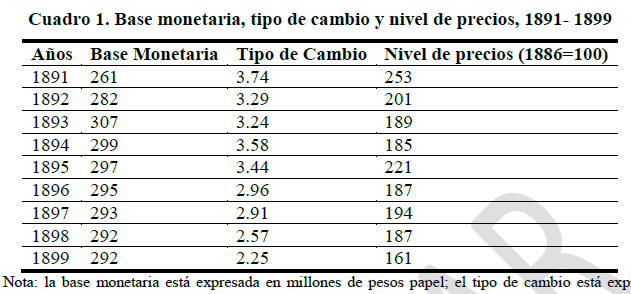
\includegraphics[scale=0.75]{uni1_cdc01}
  \caption[bpe]{Base monetaria, tipo de cambio y precios,
    1891-99. Fuente: Gomez (2014)}
  \label{fig:uni1_01}
\end{figure} 
  \end{frame}



   \begin{frame}\frametitle{La Caja de Conversión (cont.)}
    \begin{itemize}\itemsep 10pt
      \item Este primer período de ``adecuación'' ve una baja del tipo
        de cambio y de los precios. Había dos debates principales en
        esta epoca atento a la situación de deflación
        \item Primero, la paridad a la que debía establecerse la nueva
          conversión --sectores urbanos preferían 1 a 1;
          exportadores/industriales preferían paridad devaluada. 
          \item Segundo, habia incertidumbre sobre el tipo y alcance
            de reformas de tipo fiscal que aseguraran credibilidad de
            la Caja de Conversión
       \end{itemize}
      \end{frame}



   \begin{frame}\frametitle{La Caja de Conversión (cont.)}
    \begin{itemize}\itemsep 10pt
      \item Ley 3871 de 1899 $\longrightarrow$ paridad fijada al valor
        de mercado del tipo de cambio (2.27 pesos papel por peso
        oro). Argentina se convierte en un sistema de \textbf{patrón
          mixto metálico-fiduciario}
        \item Cualquier variación en la cantidad de billetes en
          circulación correspondida exactamente con las variaciones en
          la cantidad de reservas metalicas (oro) en la Caja de
          Conversion
          \item Quedaban prohibidas las operaciones de mercado abierto
            (OMA) y los redescuentos $\longrightarrow$ oferta
            monetaria endógena 
       \end{itemize}
      \end{frame}


 \begin{frame}\frametitle{La Caja de Conversión (cont.)}
   \begin{block}{Fondo de conversión}
     Una diferencia con el sistema inglés es que se creaba un fondo de
     reserva metálica llamada ``Fondo de Conversión'' con el objetivo
     de respaldar los casi 300 millones de billetes en circulación. En
     otras palabras, se buscaba respaldar con reservas metálicas no
     sólo las \textbf{nuevas emisiones} sino también las
     \textbf{emisiones existentes} al tipo de cambio fijado. Los
     recursos para dotar a este fondo provendrían de: 1) utilidades
     del BNA, 2) 5\% de sobretasa impuesto a la M, 3) producto de
     venta de activos, 4) demas rentas generales
       \end{block}
      \end{frame}




 \begin{frame}\frametitle{El Banco de la Nación Argentina (BNA)}
   \begin{itemize}
\item Creado en 1891 sobre la base del Banco Nacional con un capital
  de 50 millones de pesos mn que es emitido excepcionalmente por la
  Caja de Conversión (respaldado por bono público). Nació como una
  entidad pública
  \item La actividad del BNA estaba regulada $\longrightarrow$
    manenter encaje de 25\% de los depositos.
    \item Gozó de derechos especiales: 1) como agente financiero del
      Gobierno nacional (sólo podía prestarle a este); 2) como ``banco
      de bancos'' --podía hacer redescuentos de documentos de otros
      bancos (préstamos entre bancos). Libertad para expandirse en el territorio nacional
    \end{itemize}
      \end{frame}


 \begin{frame}\frametitle{La Caja de Conversión (cont.)}
   \begin{block}{Fondo de conversión}
     Una diferencia con el sistema inglés es que se creaba un fondo de
     reserva metálica llamada ``Fondo de Conversión'' con el objetivo
     de respaldar los casi 300 millones de billetes en circulación. En
     otras palabras, se buscaba respaldar con reservas metálicas no
     sólo las \textbf{nuevas emisiones} sino también las
     \textbf{emisiones existentes} al tipo de cambio fijado. Los
     recursos para dotar a este fondo provendrían de: 1) utilidades
     del BNA, 2) 5\% de sobretasa impuesto a la M, 3) producto de
     venta de activos, 4) demas rentas generales
       \end{block}
      \end{frame}

 
 \begin{frame}\frametitle{La Caja de Conversión (cont.)}
\begin{figure}[htbp]\vspace{0cm}
  \centering
  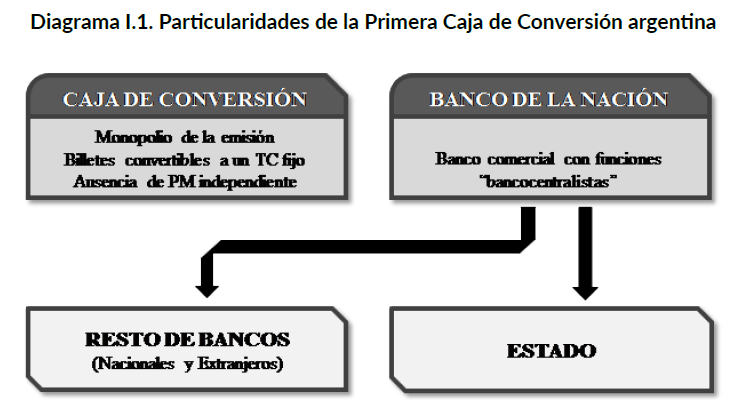
\includegraphics[scale=0.5]{uni1_cdc07}
  \caption[bpe]{Diagrama del nuevo sistema monetario. Fuente: Gomez (2018)}
  \label{fig:uni1_01}
\end{figure} 
  \end{frame}

      


  \begin{frame}\frametitle{Resumen de las reformas}
    \begin{block}{Resumen de reformas}
A mediados de 1891 paquete de medidas y reformas implementado: 1) una
significativa reforma impositiva; 2) drámatico cambio en el régimen
bancario --liquidación de dos principales bancos-; 3) centralización
de emisión monetaria en un nuevo ente; 4) renegociacion de acuerdos de
deuda. Estas reformas tendrían impacto de corto y mediano plazo
diferente en la economía argentina. 
      \end{block}
      \end{frame}


  \subsection{El desempeño en el período 1891-1899}

      
\begin{frame}\frametitle{Un cambio en las expectativas}
   \begin{itemize}
\item ¿Cómo respondió la economía argentina ante las reformas
  tentativas de 1890-91 y las nuevas reformas en esa decada?
  \item Un hecho destacable es el cambio de las expectativas por la
    futura elección de Saenz Peña $\longrightarrow$ ferviente promotor
    de austeridad fiscal
    \item La confirmación de su elección cimentó las expectativas de
      los agentes y aumentó las posibilidades de éxito del paquete de
      reformas $\longrightarrow$ primer signo fue la apreciación del
      peso papel en los mercados
    \end{itemize}
      \end{frame}

      
\begin{frame}\frametitle{La deuda externa}
   \begin{itemize}
\item Ministro de finanzas Romero  $\longrightarrow$ propone que
  Argentina pague en función de su capacidad fiscal y no a partir de
  nuevos préstamos (como era el enfoque del Empréstito de Consolidacion)
\item Logró una favorable reestructuración (``Acuerdo Romero''):
  \begin{itemize}\itemsep 10pt \medskip
    \item entre 1893-98, intereses
      sobre la mitad de stock de deuda 
      \item de 1898 en adelante, intereses sobre total del stock de
        deuda
      \item de 1901 en adelate, amortizar capital
      \end{itemize}
      \item El plan eliminaba la posibilidad de espiral explosiva de deuda
    \end{itemize}
      \end{frame}


\begin{frame}\frametitle{La deuda externa (cont.)}
   \begin{itemize}
\item Considere déficit primario real en pesos, $DEF_{t}$ financiado totalmente con
  bonos --deuda real en pesos $B_{t}$. El cambio en el stock de deuda es:
  \begin{equation*}
    B_{t}-B_{t-1}=DEF_{t}+r_{t}B_{t-1}
        \end{equation*}
\item Si el producto real, $Y_{t}$ crece a la tasa $g$ de modo que
  $Y_{t}=(1+g)Y_{t-1}$, entonces:
  \begin{equation*}
\frac{B_{t}}{Y_{t}}=\frac{1+r}{1+g}\frac{B_{t-1}}{Y_{t-1}}+\frac{1}{1+g}\frac{DEF_{t}}{Y_{t-1}}
\end{equation*}
\item que es la condición para un esquema de Ponzi si $r>g$. 
      \end{itemize}
      \end{frame}


          \begin{frame}\frametitle{La deuda externa (cont.)}
\begin{figure}[htbp]\vspace{0cm}
  \centering
  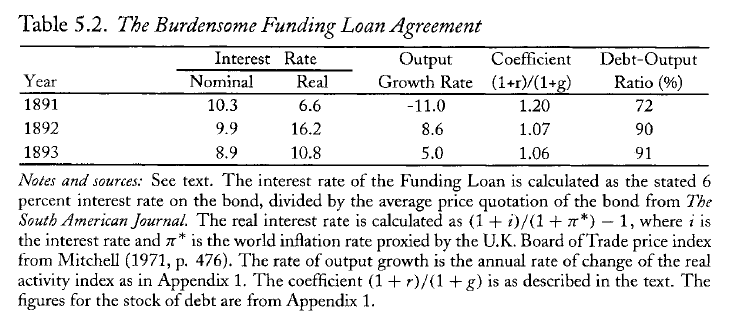
\includegraphics[scale=0.75]{uni1_fis06}
  \caption[bpe]{Servicio de la deuda - Empréstito de consolidación,
    1891-93. Fuente: Della Paolera and Taylor (2001)}
  \label{fig:uni1_01}
\end{figure} 
  \end{frame}


\begin{frame}\frametitle{La cuestión monetaria}
   \begin{itemize}
\item Romero favorecía la apreciación del tipo de cambio pero no
  quería intervenir en el mercado cambiario $\longrightarrow$ retirar
  pesos para acelerar apreciación
  \item Pero sin casi reservas de oro (ni posibilidad de
    aumentarlas) $\longrightarrow$ BM cae al 1\% promedio anual entre
    1893-99; la OM aumentó a tasas muy bajas dado que todos los bancos
    aumentaron sus encajes (legales y voluntarios)
    \item Entre 1880 y 1890, la OM creció al 21\% mientras que sólo al
      2.6\% en el período 1892-99 (ambos períodos con alta tasa de
      crecimiento real) $\longrightarrow$ PM siguió una
      \textit{Friedman rule}
    \end{itemize}
      \end{frame}


     
          \begin{frame}\frametitle{La cuestión monetaria (cont.)}
\begin{figure}[htbp]\vspace{0cm}
  \centering
  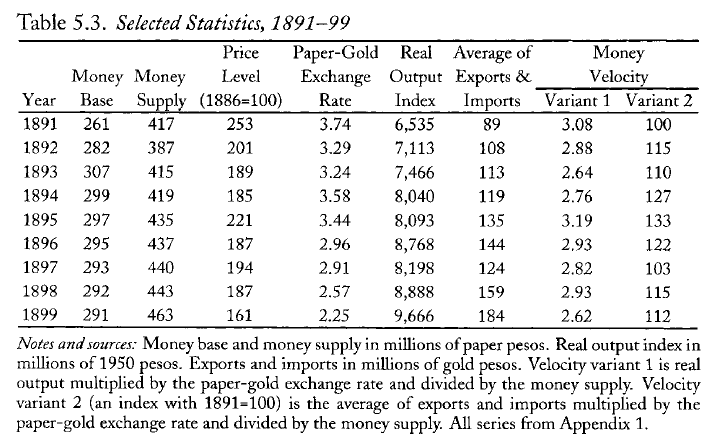
\includegraphics[scale=0.5]{uni1_refmon01}
  \caption[bpe]{Ratios monetarios, 1891-99. Fuente: Della Paolera and Taylor (2001)}
  \label{fig:uni1_01}
\end{figure} 
  \end{frame}


\begin{frame}\frametitle{Recuperación vía deflación}
   \begin{itemize}
\item La tasa de crecimiento del producto real de Argentina en esta
  década fue del 5\% --bastante más baja que la tasa del 8.5\% en la década
  de 1880s y levemente inferior a la del periodo 1900-193
  \item En 1892, con nuevas expectativas habían aumentado las
    transacciones y con una oferta monetaria relativamente estable,
    sólo era compatible con una fuerta baja del nivel de P (21\%)
    --notese $M.V=P.Y$
    \item Esto tambien causo una apreciación del peso papel
      $\longrightarrow$ fluctúo entre 3.2 y 3.6 (1892-94) y luego cayó
      a 2.27 en 1899 --en un regimen de flotación pura
    \end{itemize}
      \end{frame}




          \begin{frame}\frametitle{Recuperación vía deflación (cont.)}
\begin{figure}[htbp]\vspace{0cm}
  \centering
  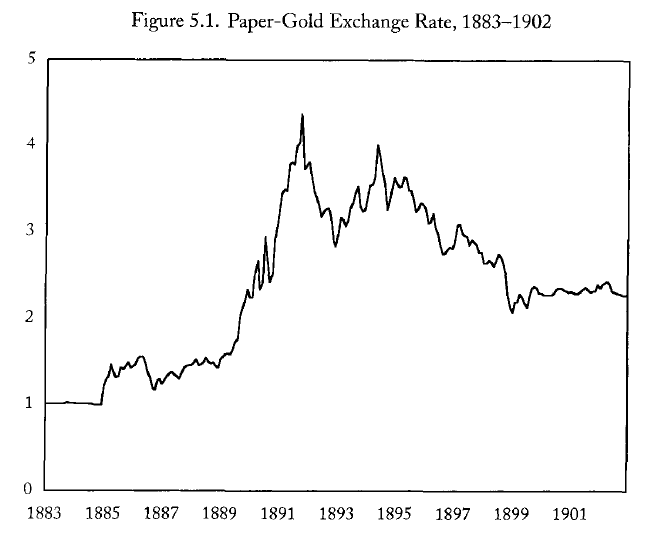
\includegraphics[scale=0.5]{uni1_refmon02}
  \caption[bpe]{Evolucion tipo de cambio papel/oro. Fuente: Della Paolera and Taylor (2001)}
  \label{fig:uni1_01}
\end{figure} 
  \end{frame}


\begin{frame}\frametitle{Recuperación vía deflación (cont.)}
   \begin{itemize}
\item La economía real se recuperó rapidamete de la crisis y creció
  aún con deflación y apreciación --importante mencionar una recesión
  y deflación de precios internacionales en 1982-94
  \item Parte importante fue la recuperación del sistema bancario
    (destruido a fines de la crisis).
    \item En 1895 se revierte fuertemente la situación internacional
      conduce a una mayor liquidez internacional y flujos de capitales
      $\longrightarrow$ los precios internos siguieron bajando pero a
      una menor tasa
    \end{itemize}
      \end{frame}




  
      
      
  \subsection{La Caja de Conversión durante el patrón oro: 1900-1913}



  \begin{frame}\frametitle{El período del patrón oro: 1900-13}
   \begin{itemize}
\item La Caja de Conversión comenzó \textbf{de hecho} sus funciones en
  1899 --coincidió con uno de los períodos más espectaculares de
  crecimiento y expansión mundial
  \item Fenomenal crecimiento de las exportaciones (``boom de cereales
    y carnes'') $\longrightarrow$ crecimiento
    anual promedio del 10\% --aumento de produccion entre 1890-1913
    y aumento de TIE en 1900-13
    \item Esto favoreció a generar saldos favorables para reestablecer
      la cuenta capital $\longrightarrow$ saldo positivo a partir de 1901
    \end{itemize}
      \end{frame}



       \begin{frame}\frametitle{El periodo del patrón oro: 1900-13 (cont.)}
\begin{figure}[htbp]\vspace{0cm}
  \centering
  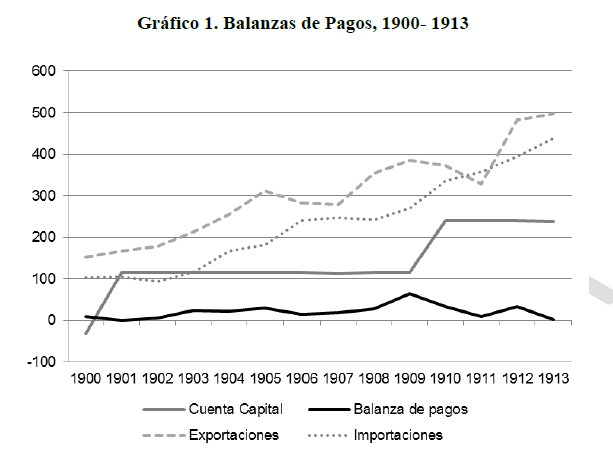
\includegraphics[scale=0.55]{uni1_cdc02}\vspace{-0.25cm}
  \caption[bpe]{Balanza de pagos. Fuente: Gomez (2014)}
  \label{fig:uni1_01}
\end{figure} 
  \end{frame}


 \begin{frame}\frametitle{El período del patrón oro: 1900-13 (cont.)}
   \begin{itemize}
\item En este período la CdC funcionó de manera esperada aunque recién
  en 1902 alcanzó la paridad estipulada $\longrightarrow$ 2.27 pesos
  papel por peso oro
  \item Una evidencia de que la CdC funcionó como una verdadera caja
    de conversión con política monetaria endógena es si uno observa la
    relación entre las variaciones en la base monetaria (BM) y las
    reservas metálicas
    \item El mismo resultado se obtiene corriendo un modelo de
      regresión sencillo entre BM y reservas
    \end{itemize}
      \end{frame}
  

  \begin{frame}\frametitle{El periodo del patrón oro: 1900-13 (cont.)}
\begin{figure}[htbp]\vspace{0cm}
  \centering
  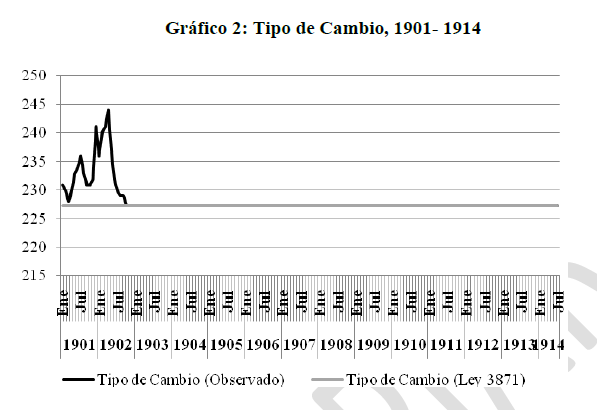
\includegraphics[scale=0.5]{uni1_cdc03}
  \caption[bpe]{Tipo de cambio nominal. Fuente: Gomez (2014)}
  \label{fig:uni1_01}
\end{figure} 
  \end{frame}
      


  
  \begin{frame}\frametitle{El periodo del patrón oro: 1900-13 (cont.)}
\begin{figure}[htbp]\vspace{0cm}
  \centering
  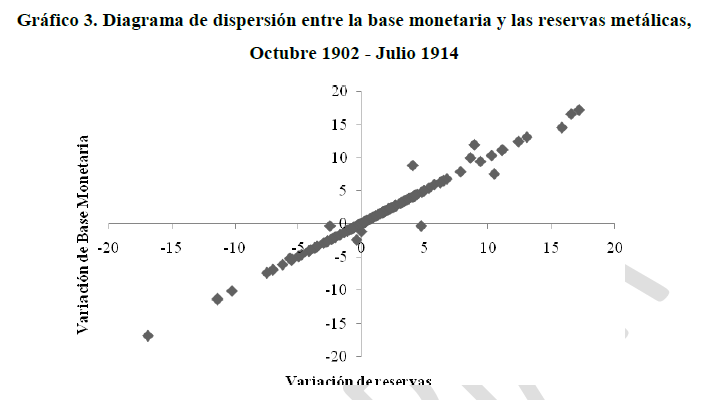
\includegraphics[scale=0.5]{uni1_cdc04}
  \caption[bpe]{Base monetaria y reservas metalicas. Fuente: Gomez (2014)}
  \label{fig:uni1_01}
\end{figure} 
  \end{frame}


 \begin{frame}\frametitle{El período del patrón oro: 1900-13 (cont.)}
   \begin{itemize}
\item Durante este período el \textbf{sistema monetario} funcionó
  correctamente y sirvio para dar previsibilidad y confianza a los
  actores económicos $\longrightarrow$ acompañó y potenció al
  crecimiento del sistema real (bienes y servicios)
  \item ¿Qué pasó con el Fondo de Conversión? Pasó de 140 mil pesos
    oro en 1902 a 30 millones en en 1910
    \item De esta manera, el respaldo en pesos oro de la BM llegó a
      ser del 73\%
    \end{itemize}
      \end{frame}



  
  \begin{frame}\frametitle{El periodo del patrón oro: 1900-13 (cont.)}
\begin{figure}[htbp]\vspace{0cm}
  \centering
  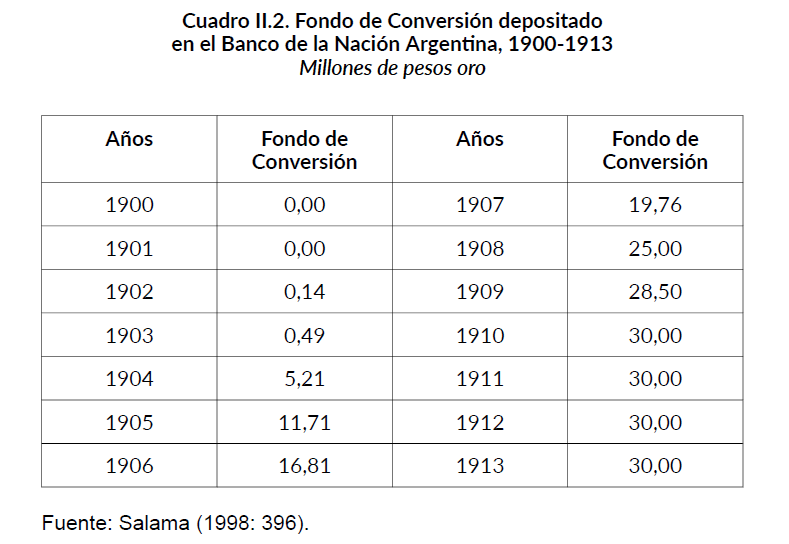
\includegraphics[scale=0.5]{uni1_cdc05}
  \caption[bpe]{El Fondo de Conversion. Fuente: Gomez (2014)}
  \label{fig:uni1_01}
\end{figure} 
  \end{frame}

      

      
  
  \begin{frame}\frametitle{El periodo del patrón oro: 1900-13 (cont.)}
\begin{figure}[htbp]\vspace{0cm}
  \centering
  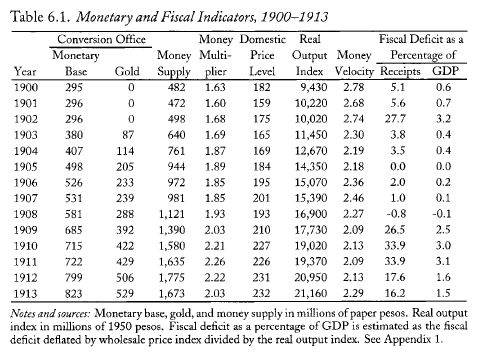
\includegraphics[scale=0.7]{uni1_cdc06}\vspace{-0.25cm}
  \caption[bpe]{Base monetaria y otros indicadores, 1900-13. Fuente:
    Della Paolera and Taylor (2001)}
  \label{fig:uni1_01}
\end{figure} 
  \end{frame}

      
\begin{frame}\frametitle{El período del patrón oro: 1900-13 (cont.)}
   \begin{itemize}
   \item BNA fue una entidad financieramente solida en todo este
     período --tuvo un crecimiento promedio anual de depósitos de casi
     el 15\% y un ratio de reservas/depositos de casi el 50\%
     \item El resto de los bancos emularon este comportamiento aunque
       en menor medida --crecimento medio anual del 5.5\% y liquidez
       (ratio R/D de 33\%)
       \item El ultimo actor de importancia --el Estado- tuvo un
         comportamiento dispar. Alternó déficits y superavits en este periodo
   \end{itemize}
      \end{frame}



   
  
  \begin{frame}\frametitle{El periodo del patrón oro: 1900-13 (cont.)}
\begin{figure}[htbp]\vspace{0cm}
  \centering
  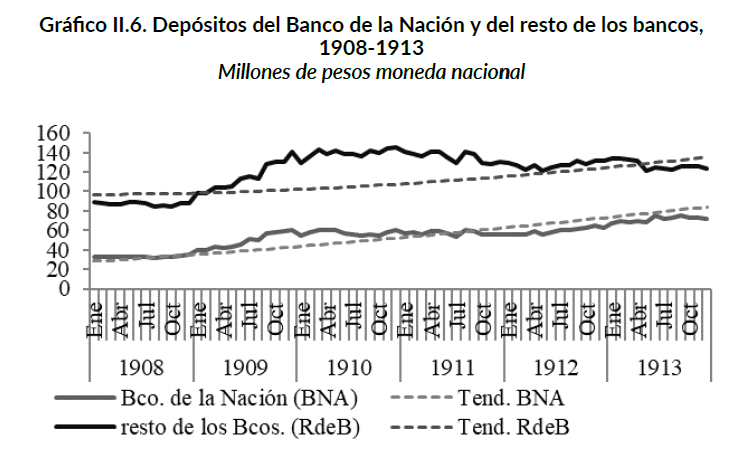
\includegraphics[scale=0.5]{uni1_bancos01}\vspace{-0.25cm}
  \caption[bpe]{Evolución depositos bancarios. Fuente: Gomez (2018))}
  \label{fig:uni1_01}
\end{figure} 
  \end{frame}



   
  
  \begin{frame}\frametitle{El periodo del patrón oro: 1900-13 (cont.)}
\begin{figure}[htbp]\vspace{0cm}
  \centering
  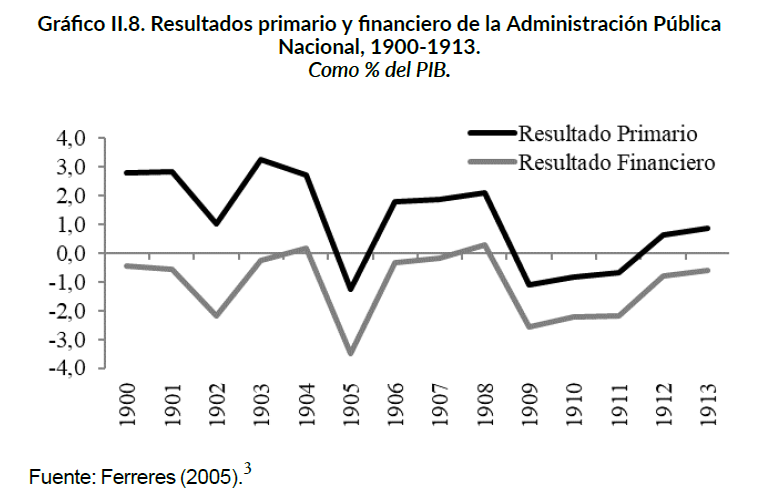
\includegraphics[scale=0.5]{uni1_bancos02}\vspace{-0.25cm}
  \caption[bpe]{Resultados primario y financiero del Estado. Fuente: Gomez (2018))}
  \label{fig:uni1_01}
\end{figure} 
  \end{frame}


  
   
  
  \begin{frame}\frametitle{El periodo del patrón oro: 1900-13 (cont.)}
\begin{figure}[htbp]\vspace{0cm}
  \centering
  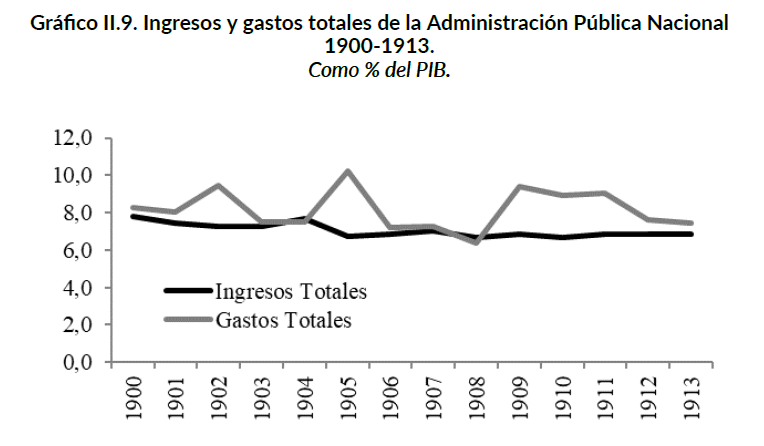
\includegraphics[scale=0.5]{uni1_bancos03}\vspace{-0.25cm}
  \caption[bpe]{Evolución ingresos y gastos del Estado. Fuente: Gomez (2018))}
  \label{fig:uni1_01}
\end{figure} 
  \end{frame}



  \begin{frame}\frametitle{El período del patrón oro: 1900-13 (cont.)}
   \begin{itemize}
   \item Si bien los ingresos totales (como proporcion de PBI) fueron
     casi constantes alrededor de 8\% puede verse que los gastos
     flucturan en ciertos momentos puntuales --1902, 1905 y 1909.
     \item Estos saltos se debían a tres factores esencialmente: 1)
       inversiones y obras públicas; 2) pensiones y jubilaciones; 3)
       pago de letras del prestamo Baring
       \item Pero puede observarse que en general en este periodo no
         se produce una aceleración en el deterioro de las cuentas
         fiscales que hubiera requerido de fuertes ayudas al fisco
   \end{itemize}
      \end{frame}




  \begin{frame}\frametitle{El período del patrón oro: 1900-13 (cont.)}
   \begin{itemize}
   \item En este periodo el BNA tuvo dos roles principales:
     \begin{itemize}\itemsep 10pt \medskip
     \item Sostén financiero del resto de bancos (redescuentos)
       \item Sostén financiero del Gobierno nacional 
       \end{itemize}
       \item En lo primero, hubo un aumento en la cantidad de
         prestamos a bancos pero esto fue minimo como fracción de las
         reservas de los otros bancos.
         \item En otras palabras, la liquidez de los bancos no
           dependía del BNA
   \end{itemize}
      \end{frame}



  
  \begin{frame}\frametitle{El periodo del patrón oro: 1900-13 (cont.)}
\begin{figure}[htbp]\vspace{0cm}
  \centering
  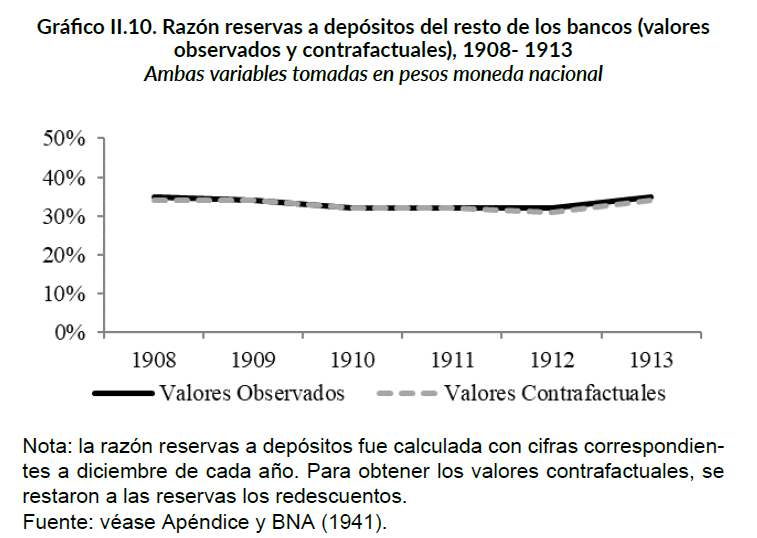
\includegraphics[scale=0.5]{uni1_bancos04}\vspace{-0.25cm}
  \caption[bpe]{Contrafactual - Reservas con y sin ayuda del BNA. Fuente: Gomez (2018))}
  \label{fig:uni1_01}
\end{figure} 
  \end{frame}


  \begin{frame}\frametitle{El período del patrón oro: 1900-13 (cont.)}
   \begin{itemize}
   \item Tampoco fue importante el rol de prestamista del Estado --en
     este periodo las cuentas del Estado se mantuvieron relativamente
     sanas
     \item Solo en 6 años en este periodo el saldo de la cuenta de
       Tesorería resultó deudor
       \item En otras palabras, tanto en terminos de financiamiento a
         otros bancos como de financiamiento al Estado, las funciones
         banco-centeralistas que tenía otorgadas el BNA no fueron necesarias
   \end{itemize}
      \end{frame}


 
  \begin{frame}\frametitle{El periodo del patrón oro: 1900-13 (cont.)}
\begin{figure}[htbp]\vspace{0cm}
  \centering
  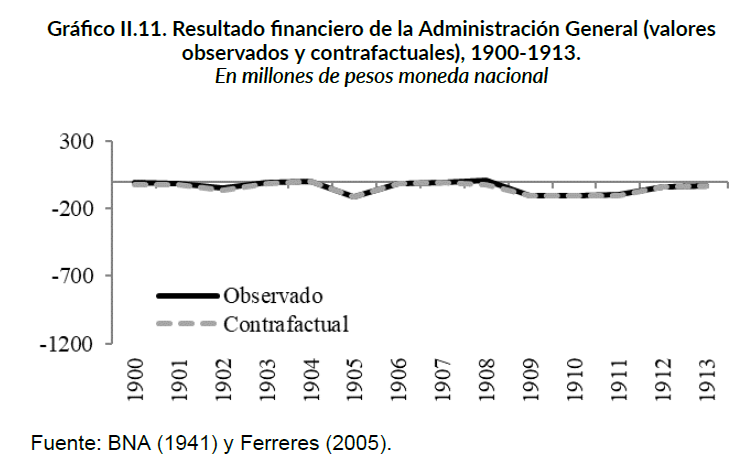
\includegraphics[scale=0.5]{uni1_bancos05}\vspace{-0.25cm}
  \caption[bpe]{Contrafactual - Resultado financiero con y sin ayuda del BNA. Fuente: Gomez (2018))}
  \label{fig:uni1_01}
\end{figure} 
  \end{frame}


    \begin{frame}\frametitle{El período del patrón oro: 1900-13 (cont.)}
   \begin{itemize}
   \item El aumento acelerado de X y el reestablecimiento de las
     entradas de K hicieron posible una \textbf{balanza de pagos positiva} en
     todo el periodo
     \item Esto permitió que Argentina pudiera operar con una tipo de
       cambio fijo desde 1902 y con moneda convertible
       \item Esto a su vez permitió el desarrollo y funcionamiento de
         un sistema bancario sólido --liquidez y tamaño- y sin necesidad de recurrir a
         funciones banco-centralistas del BNA (que tenía una solidez
         impecable)
         \item Cualquier deficit publico se cubria con deuda
   \end{itemize}
      \end{frame}


      
       
        \end{document}

        